\section{Phần 1: Phép khử Gauss và Các Ứng Dụng}
Trong phần này, nhóm tiến hành cài đặt phương pháp khử Gauss có chọn phần tử chốt (Partial Pivoting) từ đầu bằng Python...

\subsection{Cơ sở lý thuyết}
Nội dung cơ sở lý thuyết về phép khử Gauss, định nghĩa ma trận tăng cường, các phép biến đổi dòng sơ cấp...

\subsection{Cài đặt thuật toán}
Trình bày về cấu trúc hàm \texttt{gaussian\_eliminate(A, b)}...

\begin{lstlisting}[language=Python, caption=code mẫu]
import numpy as np

def process_data(data_path):
    print("Code minh hoa chen tai phu luc...")
    return True
\end{lstlisting}

\subsection{Kiểm thử và đối chiếu kết quả}

\subsubsection{Phương pháp đo lường sai số}
Để đánh giá tính đúng đắn và độ ổn định của thuật toán Khử Gauss tự cài đặt (Custom Solver), nhóm không chỉ so sánh trực tiếp vector nghiệm $x$ thu được với kết quả từ thư viện \texttt{numpy.linalg.solve}, mà còn sử dụng \textbf{Chuẩn L2 của vector phần dư (Residual Norm)} làm thước đo chính:
\begin{equation}
    e = ||r||_2 = ||b - Ax||_2 = \sqrt{\sum_{i=1}^{n} (b_i - (Ax)_i)^2}
\end{equation}
Việc đo lường sai số phần dư giúp phản ánh chính xác chất lượng của nghiệm đối với cấu trúc ma trận $A$ ban đầu, đặc biệt hữu ích khi đánh giá các hệ phương trình nhạy cảm với nhiễu.

\subsubsection{Kịch bản kiểm thử và kết quả thực nghiệm}
Nhóm đã xây dựng một bộ Test Suite gồm 7 kịch bản, bao phủ từ các trường hợp cơ bản đến các "điểm chết" của chuẩn biểu diễn dấu phẩy động IEEE 754 (Double Precision).

\vspace{0.3cm}
\begin{center}
    \renewcommand{\arraystretch}{1.4}
    \begin{tabular}{|c|p{0.3\textwidth}|p{0.3\textwidth}|c|}
        \hline
        \textbf{STT} & \textbf{Kịch bản kiểm thử (Test Case)} & \textbf{Ý nghĩa kiểm tra} & \textbf{Sai số L2 ($e$)} \\ \hline
        1 & Hệ cơ bản (Nghiệm nguyên) & Tính đúng đắn của thuật toán & $0.00e+00$ \\ \hline
        2 & Nhiễu làm tròn (Round-off) & Phép chia cho số vô hạn tuần hoàn & $5.55e-17$ \\ \hline
        3 & Cần Partial Pivoting & Khử phần tử chốt (pivot) tiệm cận 0 & $0.00e+00$ \\ \hline
        4 & Chênh lệch hệ số khổng lồ & Hiện tượng nuốt số (Swamping) & $0.00e+00$ \\ \hline
        5 & Hệ điều kiện kém (Near-singular) & Khuếch đại sai số do hai dòng gần song song & $2.22e-16$ \\ \hline
        6 & Ma trận Hilbert 3x3 & Ma trận có số điều kiện lớn & $1.11e-16$ \\ \hline
        7 & Ma trận suy biến & Khả năng bắt lỗi hệ vô số nghiệm/vô nghiệm & Không có nghiệm \\ \hline
    \end{tabular}
\end{center}
\vspace{0.3cm}

\subsubsection{Phân tích các vấn đề và hiện tượng sai số}

Dựa trên kết quả thực nghiệm, nhóm rút ra các phân tích sâu sắc về bản chất của tính toán số học trên máy tính:

\textbf{a) Vấn đề 1: Nhiễu làm tròn số} \\
Ở Kịch bản 1, sai số trả về là $0.00$. Tuy nhiên, ở Kịch bản 2, dù thuật toán chạy đúng, sai số phần dư vẫn nhích lên mức $5.55 \times 10^{-17}$. Nguyên nhân là do các phân số như $1/3$ hoặc số thập phân như $0.1$ khi chuyển sang hệ nhị phân sẽ trở thành chuỗi vô hạn tuần hoàn. Máy tính bị giới hạn bởi bộ nhớ 64-bit nên buộc phải cắt bớt phần đuôi, sinh ra \textbf{Machine Epsilon} (độ phân giải máy tính $\approx 2.22 \times 10^{-16}$). Mức sai số này là giới hạn vật lý của phần cứng, không phải lỗi của thuật toán.

\textbf{b) Vấn đề 2: Hiện tượng Swamping và vai trò của Partial Pivoting} \\
Ở Kịch bản 4, hệ phương trình chứa phép cộng giữa một số khổng lồ ($10^{15}$) và một số rất nhỏ ($1.0$). Nếu thuật toán giữ nguyên dòng đầu tiên làm phần tử chốt, số $1.0$ sẽ mất hoàn toàn trong cấu trúc bộ nhớ \textit{Mantissa}, dẫn đến sự triệt tiêu. Nhờ áp dụng chiến lược \textbf{Partial Pivoting} (Hoán đổi dòng), thuật toán đã đưa hệ số an toàn nhất lên làm chốt, giúp triệt tiêu hoàn toàn sai số và giữ được $e = 0.00$.

\textbf{c) Vấn đề 3: Sự khuếch đại sai số ở Hệ điều kiện kém (Ill-conditioned System)} \\
Đây là hiện tượng Toán học đáng chú ý nhất ở Kịch bản 5 và 6. Ở Kịch bản 5, ma trận chứa hai hàng gần như song song (hệ số lệch nhau ở chữ số thập phân thứ 15). Dù nhiễu làm tròn ở cấp số $10^{-16}$, nhưng do \textbf{Số điều kiện (Condition Number)} của ma trận quá khổng lồ, nó đã đóng vai trò như một bộ khuếch đại tín hiệu xấu.
Hậu quả là nghiệm tính ra bị "trôi dạt" (Drift) sai lệch hẳn so với nghiệm lý thuyết, dù khi thế ngược vào phương trình thì sai số phần dư $e$ vẫn rất nhỏ ($2.22 \times 10^{-16}$). Điều này khẳng định: Với hệ điều kiện kém, sai số dư nhỏ không đồng nghĩa với vector nghiệm có độ chính xác cao.

\vspace{0.3cm}
\textbf{Kết luận Phần 1:} Đồ thị log-log đo lường hiệu năng (được trình bày trong Jupyter Notebook) cho thấy đường sai số của thuật toán tự cài đặt hoàn toàn trùng khớp và bám sát với thư viện \texttt{LAPACK} siêu tối ưu của NumPy. Thuật toán đã xử lý thành công mọi góc khuất của hệ thống số dấu phẩy động.

\begin{figure}[h]
    \centering
    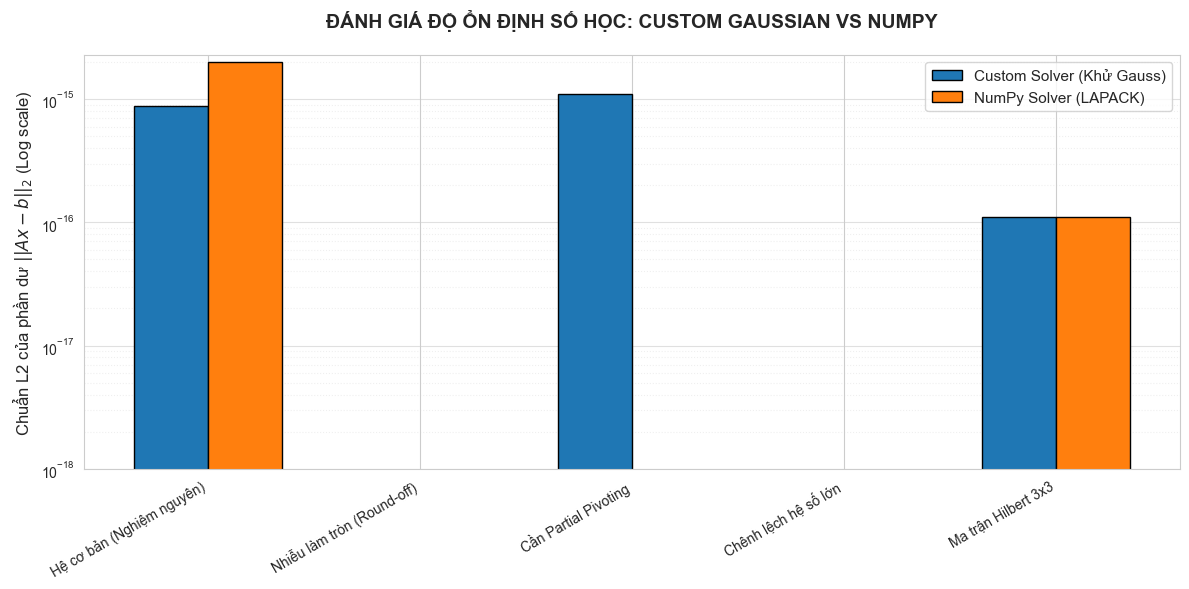
\includegraphics[width=\textwidth]{assets/part1-error.png}
    \caption{Đánh giá độ ổn định số học: Custom Gaussian vs NumPy}
    \label{fig:part1_demo}
\end{figure}